% Netzwerkanltung für die Studentenstadt Freimann
% Tex initially created by Maximilian Engelhardt <maximilian.engelhardt@stusta.mhn.de>

%\documentclass[a4paper,12pt,draft]{scrartcl}
\documentclass[a4paper,12pt]{scrartcl}

\usepackage[utf8]{inputenc}
\usepackage{ngerman}
\usepackage{eurosym}
\usepackage{tabularx}
\usepackage[pdftex,final]{graphicx}
\usepackage{wrapfig}
\usepackage[top=1.5cm,bottom=2.5cm,left=1.5cm,right=1.5cm]{geometry}
%\usepackage[margin=2cm]{geometry}
\usepackage{hyperref}


\title{Wohnanlage Studentenstadt Freimann:\\
       Anleitung zum Einrichten des Internetzugangs}
\date{\today}

\begin{document}

\maketitle

\begin{figure}[t!]
   \centering
   \vspace{-20pt}
   
\includegraphics[width=0.8\textwidth,keepaspectratio]{Bilder/StuStaNet_Logo}
   \vspace{-20pt}
\end{figure}

\section*{Allgemeine Informationen zum Netzwerkanschluss}

Dies ist eine Beschreibung, wie Sie ihren Computer an das Netzwerk der Studentenstadt anschließen können. Lesen Sie bitte vorher die Benutzerordnung gründlich durch, die Sie mit ihrem Mietvertrag erhalten haben.

Sie benötigen einen Computer mit Ethernet-Netzwerkanschluss (in allen modernen Computern integriert) und ein Netzwerkkabel zum Anschluss des Computers an der im Zimmer angebrachten Netzwerkdose. Netzwerkkabel können im Fachhandel oder auch in der Sprechstunde des StuStaNet~e~V. (siehe weiter unten) erworben werden.

Jeder, der seinen Computer an das Netzwerk der Studentenstadt anschließt, ist dafür verantwortlich, dass dadurch keine anderen Rechner im Netzwerk gefährdet werden. Dazu gehört, dass der Rechner vor Virenbefall und anderer Schadsoftware geschützt wird. Deshalb sind folgende Punkte genau zu beachten:
\begin{itemize}
    \item zeitnahes Einspielen aller verfügbaren Sicherheitsupdates für das Betriebssystem
    \item Betrieb eines Virenscanners mit allen aktuellen Updates
    \item Betrieb einer Personal Firewall, z.~B. Windows Firewall
\end{itemize}
Falls ein Rechner Auffälligkeiten aufgrund von Virenbefall zeigt, wird der zugehörige Anschluss sofort gesperrt.

\begin{em}
Bei wiederholtem Auftreten wird der Anschluss permanent außer Betrieb genommen.
\end{em}

Diese drastischen Maßnahmen sind leider notwendig, da unserem Netzwerk durch Schadsoftware enormer Schaden zugefügt wird. Das Leibniz-Rechenzentrum, das unsere Internetanbindung bereitstellt, sperrt bei erkanntem Virenbefall die Internetanbindung der gesamten Studentenstadt.

\emph{Bitte beachten Sie:} Wer sich nicht ganz sicher ist, ob er über das komplette Know-How verfügt, das nötig ist um einen Windows-Rechner sicher zu halten, sollte dringend über den Wechsel zu einem sichereren und leichter zu administrierenden Betriebssystem wie Ubuntu (kostenloser Download: \url{http://www.ubuntu.com}) nachdenken. Dieses bietet alle Features von Windows und ist, auch für Neulinge, leichter zu bedienen.


\section*{Mitgliedschaft im StuStaNet~e.V.}

Die Mitgliedschaft im StuStaNet~e.V. kostet nur einmalig \EUR{20} und bringt viele Vorteile, beispielsweise zusätzlich zu dem für alle verfügbaren Proxy-Zugang "`echtes Internet"' über einen Masquerader, ein Emailkonto, Webspace mit PHP und Datenbank, einen Datenserver und vieles mehr\footnote{\url{http://stusta-wiki.de/Dienste}}.

Die Mitgliedschaft kann in den StuStaNet~e.V. Sprechstunden beantragt werden, welche während des Semesters montags und donnerstags zwischen 19:00 und 19:30 Uhr im Blauen Haus im Erdgeschoss, Zimmer 0028 stattfinden.

Wer sich noch mehr für unser Netzwerk und die Server interessiert oder eigene Vorschläge hat, kann Hausadministrator werden (Wahlen finden immer zu Semesterbeginn in den einzelnen Häusern statt) oder einfach mal beim Adminrat vorbeischauen. Dieser findet jeden ersten Donnerstag im Monat um 20:00 Uhr im Hackerspace\footnote{3. Stock, Haus 10, Hans-Leipelt-Str. 7} statt.

\section*{Weiterführende Informationen}

Erste Anlaufstelle sollte das Stusta-Wiki und die Infoseite sein:

\begin{center}
  \begin{tabularx}{\linewidth}{|lX|}
    \hline
    \url{http://stusta-wiki.de/} & Hilfen zum Netz, Infos zum Wohnen in der Studentenstadt, Einkaufsmöglichkeiten in der Umgebung, Ärzte, Nachtleben...\\
    \hline
    \url{http://info.stusta.mhn.de/} & Ankündigungen und allgemeine Informationen über die StuSta\\
    \hline
  \end{tabularx}
\end{center}
Sollte es Probleme beim Einrichten des Internetzugangs geben, so können Sie sich außerdem an die Hausadministratoren in den einzelnen Häusern wenden. Listen der Administratoren hängen üblicherweise im Erdgeschoss aller Häuser aus.

Die Administratoren sind nur für Probleme zuständig, die das Netzwerk direkt oder indirekt betreffen. 

\newpage
\section*{Hinweise zum Sichern des Computers}

Hier ein paar kurze Hinweise zum Absichern des Computers gegen Schadsoftware.

\subsection*{Antivirenprogramme}
\paragraph*{Windows}
\begin{center}
  \begin{tabularx}{\linewidth}{|p{.2\linewidth}XX|}
    \hline
    Name & Bezugsquelle / Website & Anmerkungen\\
    \hline \hline
    Avira AntiVir & \url{http://www.free-av.com/} & kostenlos, seit 1988 am Markt\\
    \hline
    Microsoft Security Essentials & \url{http://www.microsoft.com/security\_essentials/} & kostenlos, von Microsoft, auch Antispyware\\
    \hline
    Sophos Antivirus & \url{http://sophos.lrz-muenchen.de/} & Kommerzielle Software, die vom LRZ für Studenten gratis zu beziehen ist\\
    \hline
    avast! & \url{http://www.avast.de/} & Home Edition für Privatanwender kostenlos\\
    \hline
  \end{tabularx}
\end{center}

Neben den aufgelisteten Programmen gibt es noch eine Vielzahl kommerzieller Software, deren Aufzählung den Rahmen sprengen würde. Verbreitete Anbieter sind beispielsweise Kaspersky, Norton und Bitdefender.

\paragraph*{MacOS (Apple)}
\begin{center}
  \begin{tabularx}{\linewidth}{|p{.2\linewidth}XX|}
    \hline
    Name & Bezugsquelle / Website & Anmerkungen\\
    \hline \hline
    Avira Free Mac Security & \url{https://www.avira.com/de/avira-free-mac-security} & kostenlos\\
    \hline
    Sophos Antivirus & \url{http://sophos.lrz-muenchen.de/} & Kommerzielle Software, die vom LRZ für Studenten gratis zu beziehen ist\\
    \hline
    avast! Free AV for MAC & \url{http://www.avast.com/free-antivirus-mac} & Free Edition für Privatanwender kostenlos\\
    \hline
  \end{tabularx}
\end{center}

Neben den aufgelisteten Programmen gibt es noch eine Vielzahl kommerzieller Software, deren Aufzählung den Rahmen sprengen würde. Verbreitete Anbieter sind beispielsweise Kaspersky, Norton und McAfee.

\paragraph*{Linux}

Zur Zeit ist unter diesem Betriebssystem eine Verwendung von Antivirensoftware nicht notwendig. Unter anderem aufgrund der geringeren Verbreitung und der unterschiedlichen Softwarearchitektur sind Viren (noch) kein Problem auf dieser Plattform.

\pagebreak

\subsection*{Antispywareprogramme}

Spyware ist meist unerwünschte Software, die den Benutzer ausspioniert und persönliche Daten sammelt. Weitere Informationen findet man z.B. auf Wikipedia\footnote{\url{http://de.wikipedia.org/wiki/Spyware}}.

\begin{center}
  \begin{tabularx}{\linewidth}{|p{.18\linewidth}Xp{.3\linewidth}|}
    \hline
    Name & Bezugsquelle / Website & Anmerkungen\\
    \hline \hline
    Windows Defender & \url{http://www.microsoft.com/germany/windows/products/winfamily/defender/default.mspx} & Bereits in Microsoft Security Essentials integriert\\
    \hline
    Spybot – Search \& Destroy & \url{http://www.safer-networking.org/} & Ab Windows 95, kostenlos für Privatanwender\\
    \hline
    Ad-Aware & \url{http://www.lavasoft.com/products/select\_your\_product.php} & Kostenlose Version verfügbar\\
    \hline
  \end{tabularx}
\end{center}

Neben den hier aufgelisteten kostenlosen Programmen gibt es auch diverse kommerzielle Angebote, oft in Kombination mit Personal Firewall und Antvirenprogramm.

\subsection*{Personal Firewalls}

Eine Firewall kontrolliert die Verbindung zwischen dem PC und dem Netzwerk, an dem der PC angeschlossen ist. Weitere Informationen findet man z.B. auf Wikipedia\footnote{\url{http://de.wikipedia.org/wiki/Personal\_Firewall}}.

Fast jeder Antivirus-Anbieter hat heutzutage auch eine Personal Firewall im Angebot, meist in einem Komplettpaket, das Antivirensoftware, Personal Firewall und ein Antispywareprogramm enthält.

Generell ist die Verwendung der im Betriebssystem integierten Firewall aber ausreichend.

\newpage

\section*{Netzwerkkonfiguration}

Pro Anschluss stehen 8 IP-Adressen zur Auswahl. Der jeweilige Adressbereich ist auf der Netzwerkdose zu finden. Sollte dies nicht der Fall oder der Aufkleber unlesbar sein, wenden Sie sich bitte an die Hausverwaltung.

\subsection*{Überblick}

Das Einrichten der Internetanbindung besteht aus folgenden Teilen:
\begin{itemize}
    \item Anschluss an die Netzwerkbuchse
    \item Konfiguration der Netzwerkeinstellungen im Betriebssystem
    \item Eintragen des Proxyservers bzw. -skripts im Browser
\end{itemize}


\begin{center}
  \begin{tabularx}{\linewidth}{|lXp{.2\linewidth}|}
    \hline
    Einstellung & Wert & Beispiel \\
    \hline \hline
    IP-Adresse & \nolinkurl{10.150.xxx.yyy} - \nolinkurl{10.150.xxx.zzz}, \newline 8 Adressen stehen zur Auswahl, zu finden auf der Netzwerkdose & \nolinkurl{10.150.243.16} – \nolinkurl{10.150.243.23} \\
    \hline
    Subnetzmaske & \nolinkurl{255.255.255.0} & \\
    \hline
    Standardgateway & \nolinkurl{10.150.xxx.254} \newline erste drei Blöcke wie IP-Adresse, vierter Block \nolinkurl{254} & \nolinkurl{10.150.243.254} \\
    \hline
    DNS-Server (Nameserver) & \nolinkurl{10.150.127.2} \newline \nolinkurl{10.150.125.2} & \\
    \hline
    DNS-Suffix (Domainname) & \nolinkurl{stusta.mhn.de} & \\
    \hline
    Proxyskript & \multicolumn{2}{l|}{\nolinkurl{http://wpad.stusta.mhn.de/proxy.pac}} \\
    \hline
    Proxyserver (manuell) & \multicolumn{2}{l|}{\nolinkurl{http://proxy.stusta.mhn.de:3128}} \\
    \hline
  \end{tabularx}
\end{center}

Es muss entweder das Proxyskript verwendet oder manuell der Proxyserver eingestellt werden. Die Verwendung des \emph{Proxyskripts} wird stark empfohlen!

\subsection*{Anschluss an der Netzwerkbuchse}

Verwenden Sie ausschließlich die linke Netzwerkbuchse. 

Achtung! Es ist \emph{strengstens untersagt}, Telefon, Modem, ISDN-Geräte oder Ähnliches an der linken Anschlussbuchse anzuschließen. Dadurch können massive Störungen im Netzwerk auftreten und Geräte beschädigt werden. 

\subsection*{E-Mail, Skype, ICQ, Onlinespiele, ...}

Der Internetanschluss in der Studentenstadt ist nur zur wissenschaftlichen Nutzung gedacht.

Standardmäßig ist der Internetzugang stark eingeschränkt und erlaubt nur normales Internetsurfen (Verbindungen ausschließlich über http-Proxy) sowie Verbindungen innerhalb des Münchner Wissenschaftsnetzes. Mailversand über POP3/IMAP, Instantmessenger und Onlinespiele funktionieren nur mit einer StuStaNet e.V. Mitgliedschaft (siehe oben).


\newpage
\enlargethispage{20pt}

\begin{figure}[t!]
    \raggedleft
    \vspace{-20pt}
    
\includegraphics[height=1cm,keepaspectratio]{Bilder/Ubuntu_logo}
    \vspace{-30pt}
\end{figure}

\section*{Schritt für Schritt Anleitung}
\subsection*{Einstellungen in Ubuntu}
\begin{enumerate}
    \item Öffnen Sie die Netzwerkkonfiguration durch Klick auf System $\rightarrow$ Einstellungen $\rightarrow$ Netzwerkkonfiguration.
    \item Markieren Sie nun im Reiter Kabelgebunden den entsprechenden Eintrag Ihrer Netzwerkkarte (im Normalfall eth0) und klicken Sie auf den Button Bearbeiten.
    \item Gehen Sie zum Reiter IPv4-Einstellungen und setzen Sie Methode auf Manuell.
    \item Unter Adressen klicken Sie auf den Button Hinzufügen.
      \begin{figure}[h!]
        \centering
        \begin{minipage}[c]{0.45\linewidth}
          \centering
          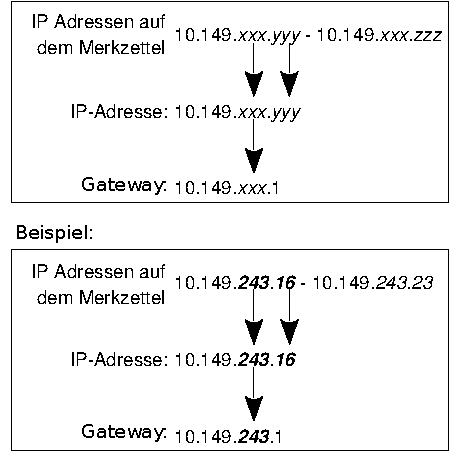
\includegraphics[width=\linewidth,keepaspectratio]{Bilder/IP_Gerneric}
        \end{minipage}
        \begin{minipage}[c]{0.5\linewidth}
          \centering
          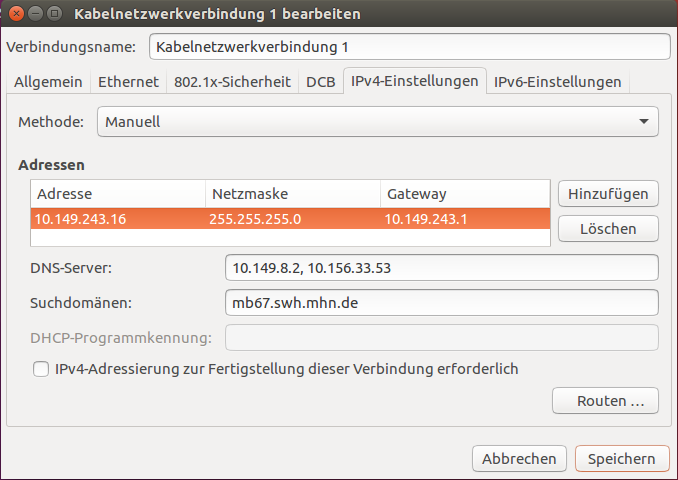
\includegraphics[width=\linewidth,keepaspectratio]{Bilder/IP_Ubuntu}
          \caption{Beispielhafte Netzwerkeinstellungen unter Ubuntu Linux}
          \vspace{-15pt}
        \end{minipage}
      \end{figure}
    \item Jetzt geben Sie IP-Adresse, Subnetzmaske, Gateway, DNS und Suchdomäne ein. Die Adressen der DNS Server lauten \nolinkurl{10.150.127.2} und \nolinkurl{10.150.125.2}, die Suchdomäne \nolinkurl{stusta.mhn.de} und die Netzmaske \nolinkurl{255.255.255.0}. Ihre jeweilige IP-Adresse steht auf einem Aufkleber auf Ihrer Anschlussbuchse bzw. auf dem Zettel, den Sie mit Ihrem Mietvertrag erhalten haben. Sollten Sie keinen Zettel mit Netzwerkdaten bekommen haben und der Aufkleber auf der Anschlussbuchse unlesbar sein, wenden Sie sich bitte an die Hausverwaltung. Bestätigen Sie mit OK und schließen Sie das Fenster für die Netzwerkeinstellungen.
\end{enumerate}
\vspace{-20pt}
\paragraph*{Proxy global einstellen}
Unter Ubuntu haben Sie die Möglichkeit, global einen Proxy zu definieren. So muss dieser nicht extra in jedem Browser eingetragen werden.
\begin{enumerate}
    \item Öffnen Sie die Netzwerk-Proxy-Einstellungen durch Klick auf System $\rightarrow$ Einstellungen $\rightarrow$ Netzwerk-Proxy.
    \item Hier markieren Sie ganz unten die Option Automatische Proxy-Konfiguration und tragen bei URL für Auto-Konfiguration: \url{http://wpad.stusta.mhn.de/proxy.pac} ein. Schließen Sie das Fenster. 
\end{enumerate}
$\rightarrow$ Der Internetzugang ist jetzt fertig konfiguriert.



\newpage
\enlargethispage{20pt}

\begin{figure}[t!]
    \raggedleft
    \vspace{-20pt}
    
\includegraphics[height=1cm,keepaspectratio]{Bilder/Windows_logo}
    \vspace{-30pt}
\end{figure}

\section*{Schritt für Schritt Anleitung}
\subsection*{Einstellungen in Windows}
\paragraph*{Windows XP}
\begin{enumerate}
     \item Öffnen Sie die Systemsteuerung durch Klick auf Start $\rightarrow$ Systemsteuerung.
     \item Klicken Sie auf Netzwerk- und Internetverbindungen.
     \item Wählen Sie im unteren Teil des Fensters den Eintrag Netzwerkverbindungen. 
     \item Markieren Sie im sich öffnenden Fenster den Eintrag LAN-Verbindung und klicken Sie links auf Einstellungen dieser Verbindung ändern.
\end{enumerate}
$\rightarrow$ Weiter bei Punkt 5.
\paragraph*{Windows Vista/7}
\begin{enumerate}
    \item Öffnen Sie die Systemsteuerung durch Klick auf Start $\rightarrow$ Systemsteuerung.
    \item Wählen Sie unter Netzwerk und Internet den Punkt Netzwerkstatus und -aufgaben anzeigen.
    \item Nach Klick auf Netzwerkverbindungen verwalten wählen Sie im darauffolgenden Fenster durch einen Rechtsklick auf LAN-Verbindung deren Eigenschaften aus.
\end{enumerate}
$\rightarrow$ Weiter bei Punkt 5.
      \begin{figure}[h!]
	\centering
        \vspace{-5pt}
        \begin{minipage}[c]{0.45\linewidth}
          \centering
          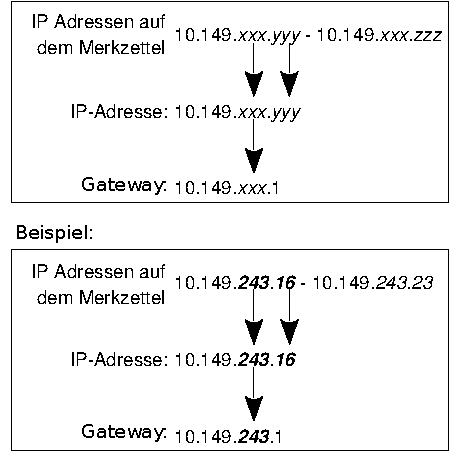
\includegraphics[width=\linewidth,keepaspectratio]{Bilder/IP_Gerneric}
        \end{minipage}
        \begin{minipage}[c]{0.48\linewidth}
          \centering
          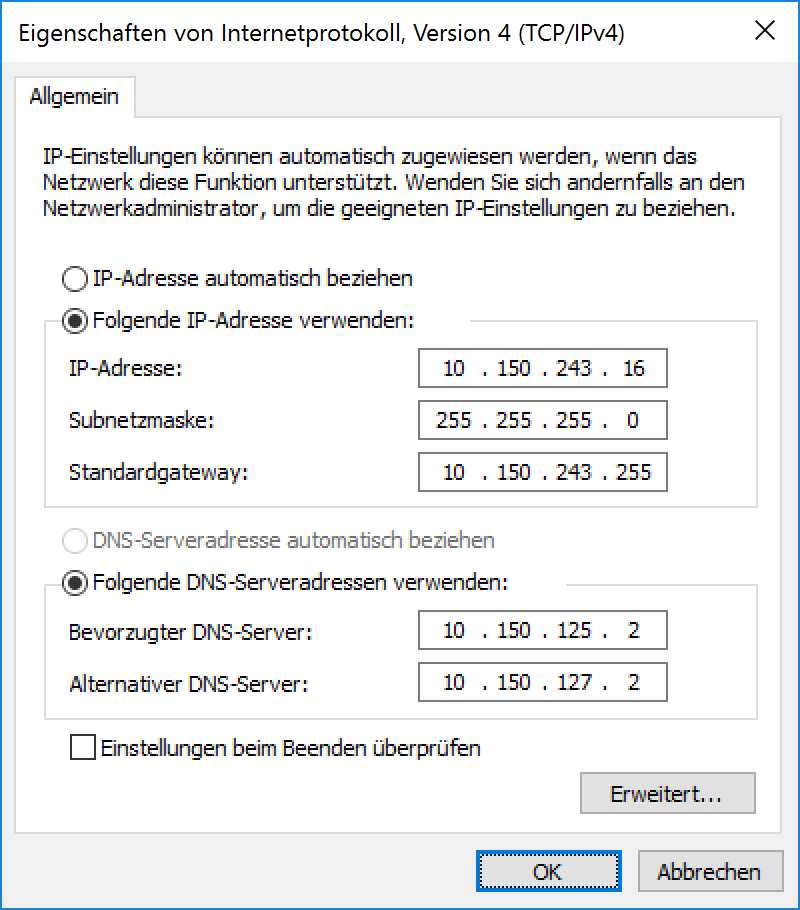
\includegraphics[width=\linewidth,keepaspectratio]{Bilder/IP_Windows}
          \caption{Beispielhafte Netzwerkeinstellungen unter Windows Vista}
        \end{minipage}
      \vspace{-20pt}
      \end{figure}
\paragraph*{Windows 8}
\begin{enumerate}
	\item Öffnen Sie die Systemsteuerung, in dem Sie die Windows-Taste drücken, \glqq Systemsteuerung\grqq  \ eingeben und ENTER drücken
	\item Wählen Sie unter Netzwerk und Internet den Punkt Netzwerkstatus und -aufgaben anzeigen.
    \item Nach Klick auf Netzwerkverbindungen verwalten wählen Sie im darauffolgenden Fenster durch einen Rechtsklick auf LAN-Verbindung deren Eigenschaften aus.
\end{enumerate}
$\rightarrow$ Weiter bei Punkt 5.

\paragraph*{Windows 10}
\begin{enumerate}
	\item Klicken Sie auf das Windowssymbol in der unteren linken Ecke und anschließend auf \emph{Einstellungen}
	\item Klicken Sie auf \textit{Netzwerk und Freigabecenter} und wählen Sie unter \textit{Verwandte Einstellungen} den Punkt \textit{Adapteroptionen ändern}. Sollten Sie diesen Punkt nicht finden können Sie auch in der Suchzeile rechts oben nach \glqq Adapteroptionen ändern\grqq suchen.
    \item Ihnen sollten nun mehrere Netzwerkverbindungen aufgelistet sein. Klicken Sie mit der \textbf{rechten} Maustaste auf \textit{Local Area Connection} und klicken Sie dann auf \textit{Eigenschaften}.
\end{enumerate}
$\rightarrow$ Weiter bei Punkt 5.

\paragraph*{Windows XP/Vista/7/8/10}
\begin{enumerate}
    \setcounter{enumi}{4}
    \item Markieren Sie den Eintrag \textit{Internetprotokoll Version 4 (TCP/IPv4)} (Windows Vista/7/8/10) bzw. Internetprotokoll  (TCP/IP) (Windows XP) und klicken Sie danach auf Eigenschaften.
    \item Jetzt geben Sie IP-Adresse, Subnetzmaske, Standardgateway und DNS Server ein. Die Adressen der DNS-Server lauten \textbf{10.150.127.2} und \textbf{10.150.125.2}, die Subnetzmaske \textbf{255.255.255.0}. Ihre jeweilige IP-Adresse steht auf einem Aufkleber auf Ihrer Anschlussbuchse bzw. auf dem Zettel, den Sie mit Ihrem Mietvertrag erhalten haben. Sollten Sie keinen Zettel mit Netzwerkdaten bekommen haben und der Aufkleber auf der Anschlussbuchse unlesbar sein, wenden Sie sich bitte an die Hausverwaltung.
    \item Klicken Sie auf Erweitert und wählen im folgenden Dialog den Reiter DNS aus. Tragen Sie im Feld DNS-Suffix für diese Verbindung \textbf{stusta.mhn.de} ein.
    \item Bestätigen mit OK.
\end{enumerate}
$\rightarrow$ Weiter bei den Browsereinstellungen.



\pagebreak

\begin{figure}[t!]
    \raggedleft
    \vspace{-20pt}
    
\includegraphics[height=1cm,keepaspectratio]{Bilder/OSXLeopard}
    \vspace{-30pt}
\end{figure}

\section*{Schritt für Schritt Anleitung}
\subsection*{Einstellungen in Mac OS X}
\begin{enumerate}
    \item Öffnen Sie die Netzwerkkonfiguration durch Klick auf Apfel (oben links) und wählen dann Systemeinstellungen $\rightarrow$ Netzwerk aus.
    \item Markieren Sie nun das Netzwerkgerät Ethernet.
    \item Setzen Sie das Feld IPv4 Konfigurieren auf Manuell.
    \item Jetzt geben Sie IP-Adresse, Teilnetzmaske, Gateway, DNS-Server und Such-Domains ein. Die Adressen der DNS-Server lauten \nolinkurl{10.150.127.2} und \nolinkurl{10.150.125.2}, die Such-Domains stusta.mhn.de und die Teilnetzmaske \nolinkurl{255.255.255.0}. Ihre jeweilige IP-Adresse steht auf einem Aufkleber auf Ihrer Anschlussbuchse bzw. auf dem Zettel, den Sie mit Ihrem Mietvertrag erhalten haben. Sollten Sie keinen Zettel mit Netzwerkdaten bekommen haben und der Aufkleber auf der Anschlussbuchse unlesbar sein, wenden Sie sich bitte an die Hausverwaltung. Bestätigen Sie mit Anwenden.
      \begin{figure}[h!]
      \centering
%      \vspace{-5pt}
        \begin{minipage}[c]{0.38\linewidth}
          \centering
          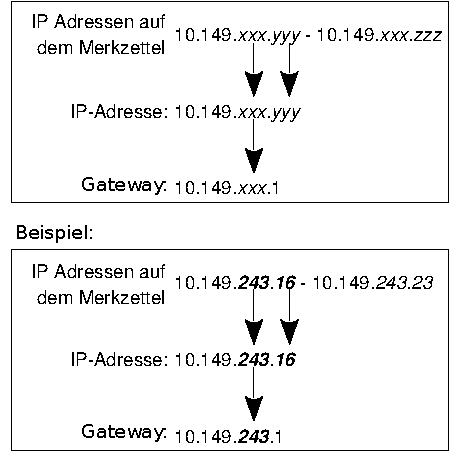
\includegraphics[width=\linewidth,keepaspectratio]{Bilder/IP_Gerneric}
        \end{minipage}
        \begin{minipage}[c]{0.60\linewidth}
          \centering
          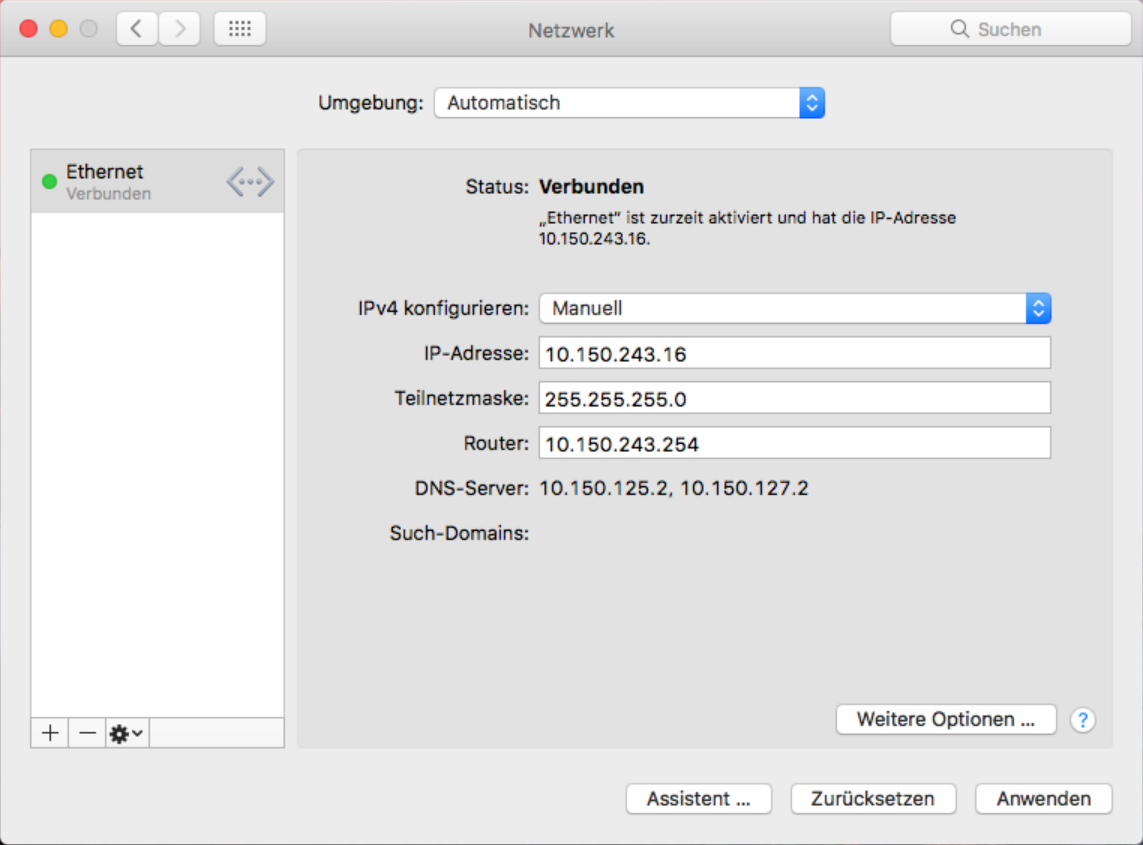
\includegraphics[width=\linewidth,keepaspectratio]{Bilder/IP_MAC}
          \caption{Beispielhafte Netzwerkeinstellungen unter Mac OS~X}
        \end{minipage}
      \vspace{-20pt}
      \end{figure}
\end{enumerate}
\vspace{-15pt}
\paragraph*{Proxy global einstellen}
Unter Mac OS X haben Sie die Möglichkeit, global einen Proxy zu definieren. So muss dieser nicht extra in jedem Browser eingetragen werden, Firefox benötigt allerdings trotzdem eine gesonderte Einstellungen (siehe Browsereinstellungen)
%\begin{wrapfigure}{r}{0.4\textwidth}
%  \vspace{-20pt}
%  \begin{center}
%    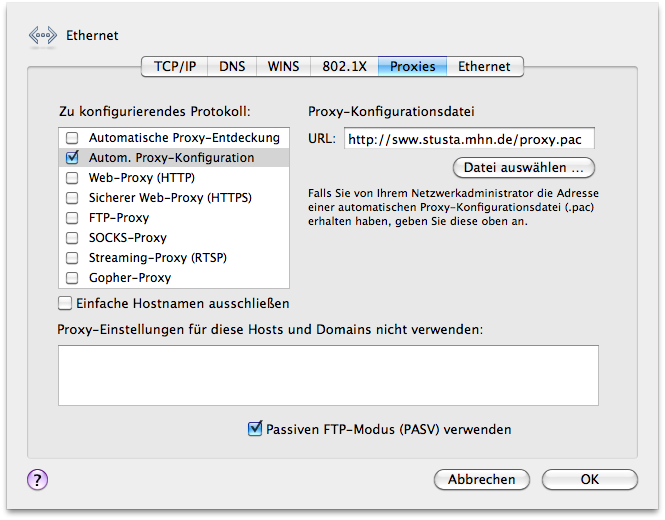
\includegraphics[width=0.48\textwidth,keepaspectratio]{Bilder/Proxy_MAC}
%  \end{center}
%  \vspace{-20pt}
%  \caption{Beispielhafte Proxyeinstellungen unter Mac OS~X}
%  \vspace{-10pt}
%\end{wrapfigure}
\begin{enumerate}
    \item Öffnen Sie mit dem Button Weitere Optionen... im voherigen Dialog die Detaileinstellungen und wechseln sie auf die Registerkarte Proxies
    \item Setzen sie bei Zu konfigurierendes Protokoll vor Autom. Proxy-Konfiguration einen Hacken und tragen rechts bei URL \url{http://wpad.stusta.mhn.de/proxy.pac} ein. Schließen Sie die Detaileinstellungen mit OK und bestätigen Sie erneut mit Anwenden. Sie können die Netzwerkeinstellungen jetzt schließen.
\end{enumerate}
$\rightarrow$ Der Internetzugang ist jetzt fertig konfiguriert.

\newpage

\section*{Browsereinstellungen}

\begin{wrapfigure}{r}{0.5\textwidth}
%  \vspace{-20pt}
  \begin{center}
    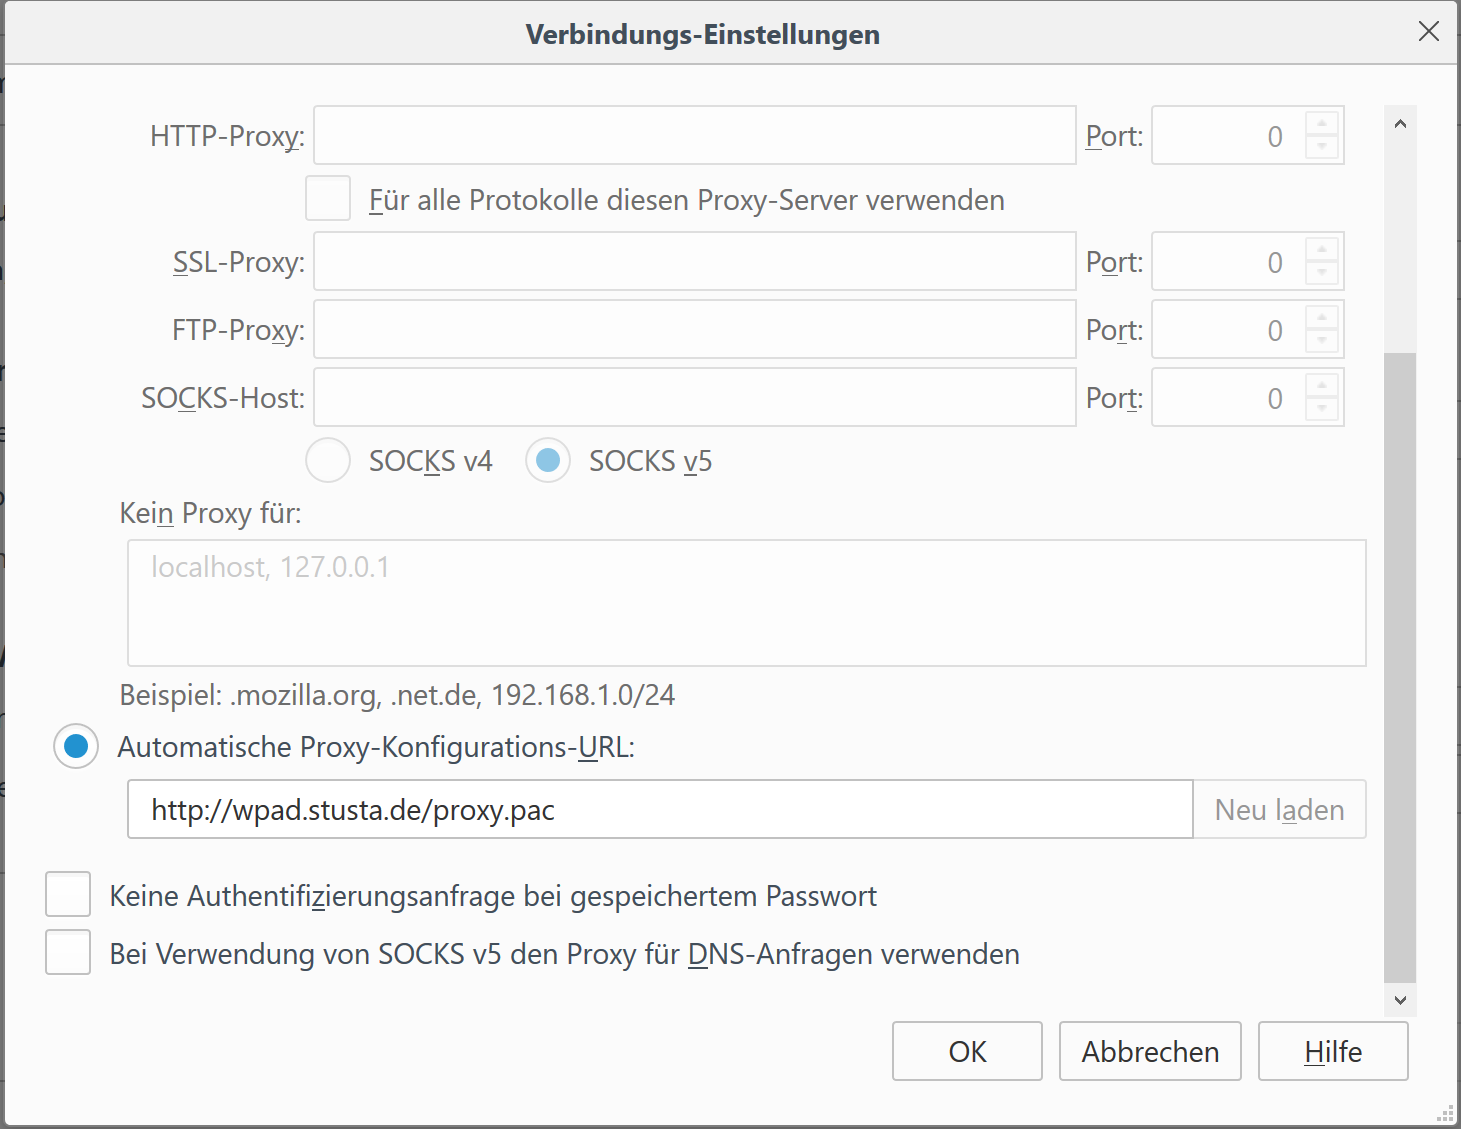
\includegraphics[width=0.5\textwidth,keepaspectratio]{Bilder/Proxy_Firefox}
  \end{center}
%  \vspace{-20pt}
  \caption{Eintragen des Proxyskripts in Mozilla Firefox}
%  \vspace{-10pt}
\end{wrapfigure}

\subsection*{
\includegraphics[height=1.2cm,keepaspectratio]{Bilder/Firefox_35_logo} Mozilla Firefox}
\begin{enumerate}
    \item Firefox starten.
    \item Wählen Sie im Untermenü Extras den Punkt Einstellungen. Unter Linux befinden sich die Einstellungen unter Bearbeiten $\rightarrow$ Einstellungen.
    \item Klicken Sie unter der Kategorie Erweitert auf den Reiter Netzwerk.
    \item Im Bereich Verbindung auf den Button Einstellungen... klicken.
    \item Markieren Sie den untersten Punkt und tragen Sie als Automatische Proxy-Konfigurations-URL: \\ \url{http://wpad.stusta.mhn.de/proxy.pac} ein.
    \item Bestätigen Sie mit OK und schließen Sie die restlichen Fenster.
\end{enumerate}
$\rightarrow$ Der Internetzugang ist nun fertig konfiguriert.


\begin{wrapfigure}{r}{0.5\textwidth}
%  \vspace{-20pt}
  \begin{center}
    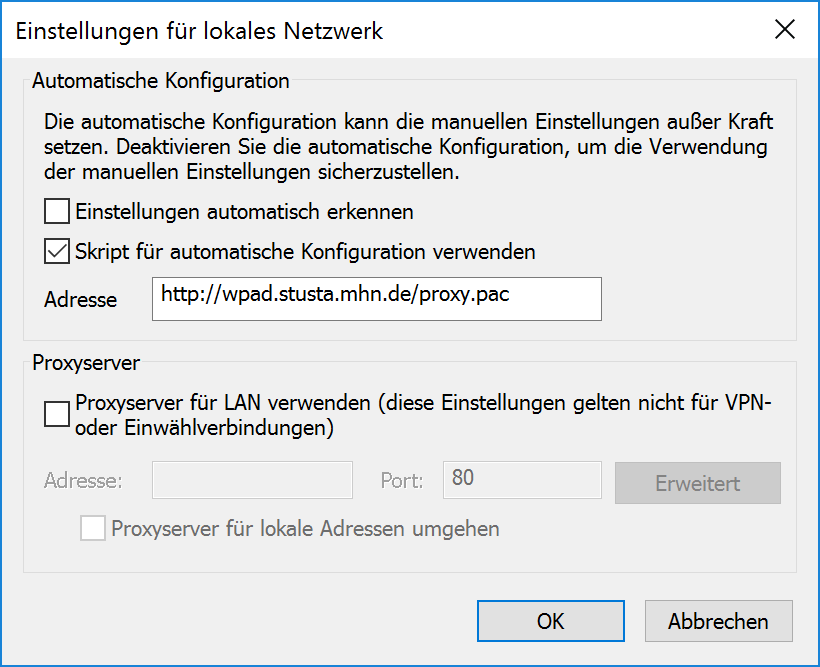
\includegraphics[width=0.5\textwidth,keepaspectratio]{Bilder/Proxy_IE}
  \end{center}
%  \vspace{-20pt}
  \caption{Eintragen des Proxyskripts im Internet Explorer}
%  \vspace{-10pt}
\end{wrapfigure}

\subsection*{
\includegraphics[height=1.2cm,keepaspectratio]{Bilder/Internet_Explorer_7_Logo} Internet Explorer}
\begin{enumerate}
    \item Internet Explorer starten.
    \item Wählen Sie im Untermenü Extras den Punkt Internetoptionen.
    \item Im Reiter Verbindungen auf den Button LAN-Ein\-stellungen klicken.
    \item Setzen Sie bei Automatisches Konfigurationsskript verwenden einen Haken und tragen Sie bei der Adresse \\ \url{http://wpad.stusta.mhn.de/proxy.pac} ein.
    \item Bestätigen Sie mit OK und schließen Sie die restlichen Fenster.
\end{enumerate}
$\rightarrow$ Der Internetzugang ist nun fertig konfiguriert.

\newpage
\begin{wrapfigure}{r}{0.5\textwidth}
%  \vspace{-20pt}
  \begin{center}
    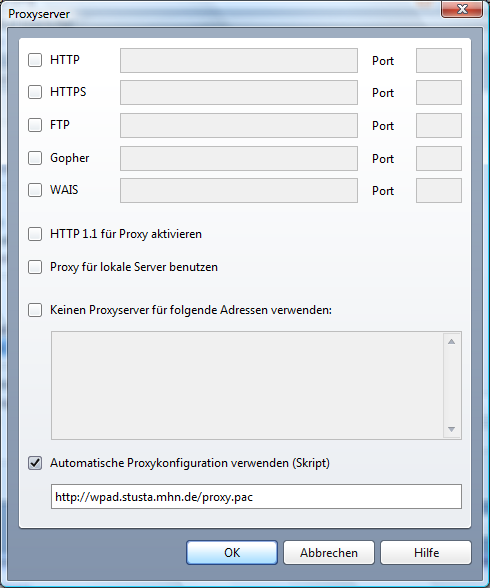
\includegraphics[width=0.5\textwidth,keepaspectratio]{Bilder/Proxy_Opera}
  \end{center}
%  \vspace{-20pt}
  \caption{Eintragen des Proxyskripts im Opera}
%  \vspace{-10pt}
\end{wrapfigure}

\subsection*{
\includegraphics[height=1.2cm,keepaspectratio]{Bilder/Opera_O} Opera}
\begin{enumerate}
    \item Opera starten.
    \item Wählen Sie im Untermenü Extras den Punkt Einstellungen...
    \item Wählen Sie im Reiter Erweitert auf der linken Seite die Kategorie Netzwerk und dann klicken Sie auf den Button Proxy.
    \item Setzen Sie bei Automatische Proxykonfiguration verwenden (Skript) einen Haken und tragen Sie \\ \url{http://wpad.stusta.mhn.de/proxy.pac} ein.
    \item Schließen Sie beide Fenster mit OK.
\end{enumerate}
$\rightarrow$ Der Internetzugang ist nun fertig konfiguriert.


\end{document}